\hypertarget{pink-floyd}{%
\section{Pink Floyd}\label{pink-floyd}}

\begin{figure}[!ht]
  \begin{adjustwidth}{-\oddsidemargin-1in}{-\rightmargin}
    \centering
    
\includegraphics[trim={0 5cm 0 2cm,}, clip, width=\paperwidth]{./S01/img/2/pink-floyd.png}
    % \caption{Pink Floyd\label{fig:pink-floyd}}
  \end{adjustwidth}
\end{figure}

\begin{tcolorbox}[enhanced,center upper,
    drop fuzzy shadow southeast, boxrule=0.3pt,
    lower separated=false, breakable,
    colframe=black!30!dialogoBorder,colback=white]
\begin{minipage}[c]{0.16\linewidth}
  \raisebox{\dimexpr-\height+\ht\strutbox\relax}{
    \centering 
\includegraphics[width=1.4cm]{./assets/img/chandler.png}
  }
   & \centering \scriptsize{Chandler}
\end{minipage}
\hfill
\begin{minipage}[c]{0.8\linewidth}
  \textbf{- ...before Pink Floyd comes out.}\\
  - ...antes do show do Pink Floyd.
\end{minipage}
\end{tcolorbox}

\saveparinfos
\noindent
\begin{minipage}[c]{0.5\textwidth}\useparinfo

Chandler menciona a banda britânica de rock progressivo \emph{Pink
Floyd}, formada em 1965 e caracterizada por ter muitos elementos visuais
no palco. A banda lança o albúm \emph{The Division Bell} em Março 1994,
um pouco antes do começo da série.\footnote{\sloppy Pink Floyd - Site oficial. \url{https://www.pinkfloyd.com/}}

\end{minipage}\hfill
\begin{minipage}[c]{0.5\textwidth}

\begin{figure}
  \centering
  \begin{tikzpicture}
    \node [inner sep=0pt] at (0,0) {
      
\includegraphics[width=0.7\textwidth,keepaspectratio]{./S01/img/2/the-division-bell.jpg}
    };
    \draw [white, rounded corners=\ClipSep, line width=\ClipSep]
    (current bounding box.north west) --
    (current bounding box.north east) --
    (current bounding box.south east) --
    (current bounding box.south west) -- cycle
    ;
    \end{tikzpicture}
    \caption{The Division Bell\label{fig:the-division-bell}}
\end{figure}

\end{minipage}

\hypertarget{threes-company}{%
\section{Three's Company}\label{threes-company}}

\begin{figure}[!ht]
  \begin{adjustwidth}{-\oddsidemargin-1in}{-\rightmargin}
    \centering
    
\includegraphics[trim={0 4cm 0 2cm,}, clip, width=\paperwidth]{./S01/img/2/threes-company.png}
    % \caption{Three’s Company\label{fig:three-s-company}}
  \end{adjustwidth}
\end{figure}

\begin{tcolorbox}[enhanced,center upper,
    drop fuzzy shadow southeast, boxrule=0.3pt,
    lower separated=false,
    colframe=black!30!dialogoBorder,colback=white]
\begin{minipage}[c]{0.16\linewidth}
  \raisebox{\dimexpr-\height+\ht\strutbox\relax}{
    \centering 
\includegraphics[width=1.4cm]{./assets/img/chandler.png}
  }
   & \centering \scriptsize{Chandler}
\end{minipage}
\hfill
\begin{minipage}[c]{0.8\linewidth}
  \textbf{- I think this is the episode of Three's Company where's there's some kind of misunderstanding.}\\
  - Acho que este é o episódio de Three's Company onde há um mal-entendido.
\end{minipage}

\medskip
\begin{minipage}[c]{0.16\linewidth}
  \raisebox{\dimexpr-\height+\ht\strutbox\relax}{
    \centering 
\includegraphics[width=1.4cm]{./assets/img/phoebe.png}
  }
   & \centering \scriptsize{Phoebe}
\end{minipage}
\hfill
\begin{minipage}[c]{0.8\linewidth}
  \textbf{- Then I've already seen this one.}\\
  - Então, eu já vi.
\end{minipage}
\end{tcolorbox}

\saveparinfos
\noindent
\begin{minipage}[c]{0.5\textwidth}\useparinfo

Chandler, Joey, Phoebe e Monica assistem a \emph{sitcom} \emph{Three's
Company} (1977-1984), conhecida no Brasil como \emph{Um é Pouco, Dois é
Bom e Três é Demais}.\footnote{\sloppy Three’s Company - Site oficial. \url{http://www.threescompany.com/}}
Conta a história de Janet e Chrissy, que dividem um apartamento em Santa
Monica e conhecem um novo colega Jack. Ele estuda gastronomia e, quando
pedem para ele provar suas capacidades, finge ser gay. Eles passam a
morar juntos e passar por desentendimentos, aventuras e brincadeiras.
Daí a piada, o \emph{plot} da história quase sempre envolve um
desentendimento.\footnote{\sloppy Three’s Company - Adoro Cinema. \url{http://www.adorocinema.com/series/serie-387/foto-detalhada/?cmediafile=21161912}}

\end{minipage}\hfill
\begin{minipage}[c]{0.5\textwidth}

\begin{figure}
  \centering
  \begin{tikzpicture}
    \node [inner sep=0pt] at (0,0) {
      
\includegraphics[width=0.7\textwidth,keepaspectratio]{./S01/img/2/threes-company-cover.jpg}
    };
    \draw [white, rounded corners=\ClipSep, line width=\ClipSep]
    (current bounding box.north west) --
    (current bounding box.north east) --
    (current bounding box.south east) --
    (current bounding box.south west) -- cycle
    ;
    \end{tikzpicture}
    \caption{Three’s Company - Cover\label{fig:three-s-company-cover}}
\end{figure}

\end{minipage}

\hypertarget{thighmaster}{%
\section{Thighmaster}\label{thighmaster}}

\begin{figure}[!ht]
  \begin{adjustwidth}{-\oddsidemargin-1in}{-\rightmargin}
    \centering
    
\includegraphics[trim={0 8cm 0 3cm,}, clip, width=\paperwidth]{./S01/img/2/thighmaster.png}
    % \caption{Thighmaster\label{fig:thighmaster}}
  \end{adjustwidth}
\end{figure}

\begin{tcolorbox}[enhanced,center upper,
    drop fuzzy shadow southeast, boxrule=0.3pt,
    lower separated=false, breakable,
    colframe=black!30!dialogoBorder,colback=white]
\begin{minipage}[c]{0.16\linewidth}
  \raisebox{\dimexpr-\height+\ht\strutbox\relax}{
    \centering 
\includegraphics[width=1.4cm]{./assets/img/chandler.png}
  }
   & \centering \scriptsize{Chandler}
\end{minipage}
\hfill
\begin{minipage}[c]{0.8\linewidth}
  \textbf{- Ugly Naked Guy got a Thighmaster.}\\
  - Peladão feio fazendo exercício!
\end{minipage}
\end{tcolorbox}

\saveparinfos
\noindent
\begin{minipage}[c]{0.5\textwidth}\useparinfo

Chandler menciona que o \emph{Ugly Naked Guy} está usando um
\emph{Thighmaster}, conhecido aparelho aeróbico usado para tonificar a
parte interna da coxa. O interessante aqui é que o \emph{Thighmaster}
está diretamente relacionado à série \emph{Three's Company}, já que
\emph{Suzanne Somers} --- que faz o papel de Chrissy na série --- é a
porta-voz oficial do produto.\footnote{\sloppy Thighmaster - Fandom Wiki. \url{https://threescompany.fandom.com/wiki/Suzanne_Somers#Spokeswoman_for_Thighmaster}}
\footnote{\sloppy Thighmaster - Trechos do comercial - YouTube. \url{https://www.youtube.com/watch?v=2yVeef8AnYI}}

\end{minipage}\hfill
\begin{minipage}[c]{0.45\textwidth}

\begin{figure}
  \centering
  \begin{tikzpicture}
    \node [inner sep=0pt] at (0,0) {
      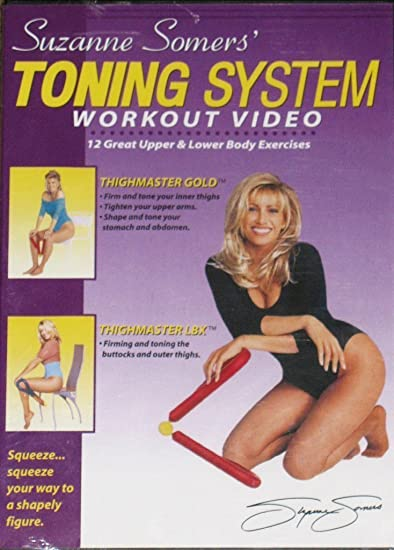
\includegraphics[width=0.8\textwidth,keepaspectratio]{./S01/img/2/suzanne-somers-thighmaster.jpg}
    };
    \draw [white, rounded corners=\ClipSep, line width=\ClipSep]
    (current bounding box.north west) --
    (current bounding box.north east) --
    (current bounding box.south east) --
    (current bounding box.south west) -- cycle
    ;
    \end{tikzpicture}
    \caption{Suzanne Somers - Thighmaster\label{fig:suzanne-somers-thighmaster}}
\end{figure}

\end{minipage}

\hypertarget{in-the-kitchen-with-dinah}{%
\section{In the kitchen with\ldots{}
Dinah?}\label{in-the-kitchen-with-dinah}}

\begin{figure}[!ht]
  \begin{adjustwidth}{-\oddsidemargin-1in}{-\rightmargin}
    \centering
    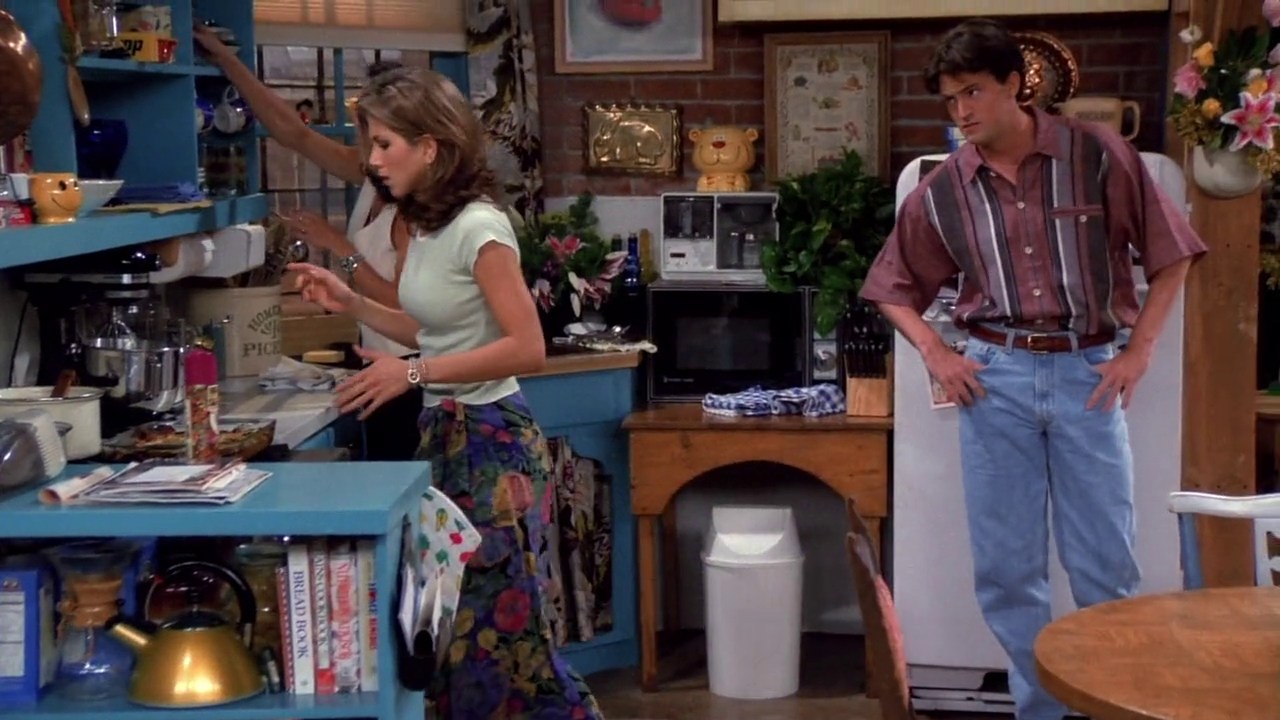
\includegraphics[trim={0 6cm 0 1cm,}, clip, width=\paperwidth]{./S01/img/2/kitchen-with-dinah.png}
    % \caption{In the kitchen with… Dinah?\label{fig:in-the-kitchen-with-dinah}}
  \end{adjustwidth}
\end{figure}

\begin{tcolorbox}[enhanced,center upper,
    drop fuzzy shadow southeast, boxrule=0.3pt,
    lower separated=false, breakable,
    colframe=black!30!dialogoBorder,colback=white]
\begin{minipage}[c]{0.16\linewidth}
  \raisebox{\dimexpr-\height+\ht\strutbox\relax}{
    \centering 
\includegraphics[width=1.4cm]{./assets/img/rachel.png}
  }
   & \centering \scriptsize{Rachel}
\end{minipage}
\hfill
\begin{minipage}[c]{0.8\linewidth}
  \textbf{- I know I had it when I was in the kitchen with...}\\
  - Sei que estava com ela na cozinha com...
\end{minipage}

\medskip
\begin{minipage}[c]{0.16\linewidth}
  \raisebox{\dimexpr-\height+\ht\strutbox\relax}{
    \centering 
\includegraphics[width=1.4cm]{./assets/img/chandler.png}
  }
   & \centering \scriptsize{Chandler}
\end{minipage}
\hfill
\begin{minipage}[c]{0.8\linewidth}
  \textbf{- Dinah?}\\
  - Dinah?
\end{minipage}
\end{tcolorbox}

Enquanto procura sua aliança, Rachel menciona que estava na cozinha, e
Chandler pergunta se ela estava com Dinah. Isso é uma alusão a canção
folclórica \emph{I've Been Working on the Railroad} (C.
1894).\footnote{\sloppy I’ve Been Working on the Railroad - Live About (Inglês). \url{https://www.liveabout.com/ive-been-working-on-the-railroad-traditional-1322525}}
\footnote{\sloppy I’ve Been Working on the Railroad - John Denver - YouTube. \url{https://www.youtube.com/watch?v=AAI6wjXEV6g}}
Segue um trecho da canção que é citado no diálogo:

\bigskip
\begin{tcolorbox}[enhanced,
    drop fuzzy shadow southeast, boxrule=0.3pt,
    lower separated=false, sidebyside, sidebyside align=top,
    halign=flush right, halign lower=left, breakable,
    colframe=black!30!dialogoBorder,colback=musicaBg]
\includegraphics[width=0.4cm]{./assets/img/icon-music.png}\\
Someone’s in the kitchen with Dinah\\Someone’s in the kitchen I know\\Someone’s in the kitchen with Dinah\\Strummin’ on the old banjo!\\
\tcblower
\includegraphics[width=0.4cm]{./assets/img/icon-language.png}\\
Alguém está na cozinha com Dinah\\Alguém está na cozinha eu sei\\Alguém está na cozinha com Dinah\\Dedilhando no velho banjo\\
\end{tcolorbox}

\hypertarget{minnie-mouse}{%
\section{Minnie Mouse}\label{minnie-mouse}}

\begin{figure}[!ht]
  \begin{adjustwidth}{-\oddsidemargin-1in}{-\rightmargin}
    \centering
    
\includegraphics[trim={0 6cm 0 1cm,}, clip, width=\paperwidth]{./S01/img/2/minnie-mouse.png}
    % \caption{Minnie Mouse\label{fig:minnie-mouse}}
  \end{adjustwidth}
\end{figure}

\begin{tcolorbox}[enhanced,center upper,
    drop fuzzy shadow southeast, boxrule=0.3pt,
    lower separated=false, breakable,
    colframe=black!30!dialogoBorder,colback=white]
\begin{minipage}[c]{0.16\linewidth}
  \raisebox{\dimexpr-\height+\ht\strutbox\relax}{
    \centering 
\includegraphics[width=1.4cm]{./assets/img/carol-1.png}
  }
   & \centering \scriptsize{Carol}
\end{minipage}
\hfill
\begin{minipage}[c]{0.8\linewidth}
  \textbf{- Minnie, if it's a girl.}\\
  - Minnie, se for menina.
\end{minipage}

\medskip
\begin{minipage}[c]{0.16\linewidth}
  \raisebox{\dimexpr-\height+\ht\strutbox\relax}{
    \centering 
\includegraphics[width=1.4cm]{./assets/img/ross.png}
  }
   & \centering \scriptsize{Ross}
\end{minipage}
\hfill
\begin{minipage}[c]{0.8\linewidth}
  \textbf{- As in Mouse?}\\
  - Minnie Mouse?
\end{minipage}
\end{tcolorbox}

Ao discutir sobre o nome de seu filho com Carol e Susan, Ross menciona
\emph{Minnie Mouse}, famosa personagem de \emph{Walt Disney} criada em
1928.\footnote{\sloppy Minnie Mouse - Wikipédia. \url{https://pt.wikipedia.org/wiki/Minnie_Mouse}}
Aparece pela primeira vez no episódio \emph{Steamboat Willie} (1928), já
como a namorada de \emph{Mickey Mouse}.\footnote{\sloppy Steamboat Willie - YouTube. \url{https://www.youtube.com/watch?v=BBgghnQF6E4}}

\hypertarget{enterprise}{%
\section{Enterprise}\label{enterprise}}

\begin{figure}[!ht]
  \begin{adjustwidth}{-\oddsidemargin-1in}{-\rightmargin}
    \centering
    
\includegraphics[trim={0 5cm 0 2cm,}, clip, width=\paperwidth]{./S01/img/2/enterprise.png}
    % \caption{Enterprise\label{fig:enterprise}}
  \end{adjustwidth}
\end{figure}

\begin{tcolorbox}[enhanced,center upper,
    drop fuzzy shadow southeast, boxrule=0.3pt,
    lower separated=false,
    colframe=black!30!dialogoBorder,colback=white]
\begin{minipage}[c]{0.16\linewidth}
  \raisebox{\dimexpr-\height+\ht\strutbox\relax}{
    \centering 
\includegraphics[width=1.4cm]{./assets/img/joey.png}
  }
   & \centering \scriptsize{Joey}
\end{minipage}
\hfill
\begin{minipage}[c]{0.8\linewidth}
  \textbf{- What are we supposed to be seeing here?}\\
  - O que deveríamos ver?
\end{minipage}

\medskip
\begin{minipage}[c]{0.16\linewidth}
  \raisebox{\dimexpr-\height+\ht\strutbox\relax}{
    \centering 
\includegraphics[width=1.4cm]{./assets/img/chandler.png}
  }
   & \centering \scriptsize{Chandler}
\end{minipage}
\hfill
\begin{minipage}[c]{0.8\linewidth}
  \textbf{- I don't know, but I think it's about to attack the Enterprise.}\\
  - Não sei, mas acho que vai atacar a Enterprise.
\end{minipage}
\end{tcolorbox}

Assistindo ao vídeo do ultrassom, Chandler faz uma piada comparando as
imagens a uma cena da séria \emph{Star Trek} (1966), e \emph{Enterprise}
é o nome da principal nave estelar. No Brasil a séria é conhecido como
\emph{Jornada nas Estrelas}.\footnote{\sloppy Star Trek - Página oficial. \url{https://intl.startrek.com/database_article/enterprise-nx-01}}

\begin{figure}
  \centering
  \begin{tikzpicture}
    \node [inner sep=0pt] at (0,0) {
      
\includegraphics[width=0.8\textwidth,keepaspectratio]{./S01/img/2/enterprise-ship.jpg}
    };
    \draw [white, rounded corners=\ClipSep, line width=\ClipSep]
    (current bounding box.north west) --
    (current bounding box.north east) --
    (current bounding box.south east) --
    (current bounding box.south west) -- cycle
    ;
    \end{tikzpicture}
    \caption{Enterprise\label{fig:enterprise}}
\end{figure}
